% \documentclass[aspectratio=43]{beamer}
\documentclass{ctexbeamer}
\usepackage[UTF8]{ctex}
\usetheme{CCNU}
\usepackage{graphicx}
\usepackage{slashed}
\usepackage{datetime}
\usepackage{biblatex}
\addbibresource{reference.bib} 
\setbeamerfont{footnote}{size=\tiny} %调整注脚的文字大小
\graphicspath{{plots/}}
\usepackage{hyperref}
\usepackage{cancel}
\usepackage{algorithm}
\usepackage{algorithmic}
\usepackage[ruled,linesnumbered]{algorithm2e}
\usepackage{algpseudocode}
\usepackage{amsmath}

\renewcommand{\algorithmicrequire}{\textbf{Input:}} 
\renewcommand{\algorithmicensure}{\textbf{Output:}}
% \usepackage{enumitem}

\usepackage{graphicx}  %%  图片包
\usepackage{subfig}    %% 子图包
\usepackage{float}     %% 浮动个数

\usepackage{hyperref}
\hypersetup{
    colorlinks=true,
    linkcolor=blue,
    filecolor=blue,      
    urlcolor=blue,
    citecolor=cyan,
}
\usepackage{tikz}
\usetikzlibrary{shapes,arrows}
\tikzstyle{startstop} = [rectangle,rounded corners, minimum width=2cm,minimum height=0.1cm,draw=black,fill=red!30]
\tikzstyle{io} = [trapezium, trapezium left angle = 70,trapezium right angle=110,minimum width=2cm,minimum height=0,1cm,text centered,draw=black,fill=blue!30]
\tikzstyle{process} = [rectangle,minimum width=3cm,minimum height=0.1cm,text centered,text width =2cm,draw=black,fill=orange!30]
\tikzstyle{decision} = [diamond,minimum width=0.1cm,minimum height=0.1cm,text centered,draw=black,aspect=3,fill=green!30]
\tikzstyle{arrow} = [thick,->,>=stealth]


\usepackage[absolute,overlay]{textpos}
\def\Put(#1,#2)#3{\leavevmode\makebox(0,0){\put(#1,#2){#3}}}

\def\mydate{\leavevmode\hbox{\the\year-\twodigits\month-\twodigits\day}}
\def\twodigits#1{\ifnum#1<10 0\fi\the#1}

\newcommand\Wider[2][3em]{%
\makebox[\linewidth][c]{%
  \begin{minipage}{\dimexpr\textwidth+#1\relax}
  \raggedright
  \centering#2
  \end{minipage}
  }
}

\def\meetingname{}

\title[\meetingname]{基于强化学习的多无人机协同草原修复方法研究 \cite{4358754} \\}
\author[X Wang]{Xianyi Wang}
\institute[LZU]{Lanzhou University}
\date[\mydate]{\meetingname\\\today}

\begin{document}
\begin{frame}[plain,t]
    \titlepage

\end{frame}
\setbeamertemplate{caption}[numbered]
%The next statement creates the title page.
\begin{frame}
    \frametitle{Contents}
    \tableofcontents
\end{frame}
%------------------------------------------------------------
\section{绪论}
\begin{frame}{研究背景与意义}
    \begin{itemize}
    \item 草原是地球上重要的生态系统,对生态和民生具有至关重要的作用。
    \item 中国草原面临退化和恶化趋势,需要保护和修复工作。
    \item 草原生态修复采用自然恢复和人工干预相结合的方式,根据地区情况进行规划。
    \item 无人机成为草原修复的重要工具,具有经济性和效率。
    \item 多无人机协同方法用于在能量有限的情况下最大化修复面积。
    \end{itemize}
    % A multiobjective optimization problem (MOP) can be stated as:
    %     \begin{align}
    %     \centering 
    %     maximize\ F(x)=(f_1(x),...,f_m(x))^T ,subject\;to\;x \in \Omega
    % \end{align}
    % \begin{itemize}
    %     \item {Decision space: $\Omega$}
    %     \item {Objective space: $R^m$ }
    %     \item {Objective function: $F:\Omega \to R^m$}
    %     \item {Pareto dominate:\ $ u \succ v\;if\ \forall i \in {1,...,m}\; u_i \ge v_i , \exists j \in {1,...,m}\;u_j > v_j$}
    %     \item Pareto optimal:$x^*,and\not\exists x\in \Omega,x \succ x^*$
    %     \item {Pareto optimal vector:$F(x^*)$}
    %     \item Pareto optimal solution set:$P^*=\{x^*|\not \exists x\in \Omega :x\succ x^*\}$
    %     \item Pareto front surface:$$PF^* = \{F(x^*)=(f_1(x^*),f_2(x^*),...,f_m(x^*))^T|x^*\in P^*\}$$
    % \end{itemize}
\end{frame}
% \subsection{国内外研究现状}
\begin{frame}{国内外研究现状}
\scriptsize
 强化学习在路径规划中的应用:
    \begin{itemize}
        \item  Liu等提出了将强化学习与遗传算法相结合,用于解决旅行商问题(TSP)。
\item Bello等构建了指针网络进行强化学习,以应对TSP问题中网络输入规模的变化。
\item Deudon等采用基于策略梯度的强化学习模型解决TSP问题。
\end{itemize}
多智能体强化学习:
\begin{itemize}
 \item 孙长银等总结了多智能体强化学习方法的原理,并讨论了闭环框架和其中的重要问题及解决方法。
\item 梁星星等探讨了多智能体强化学习中的关键技术,包括网络架构、模型鲁棒性、样本增强和对手建模等。
\end{itemize}
容量约束的车辆路径问题(CVRP):
\begin{itemize}
\item Delarue等提出了基于价值学习的强化学习框架,用于解决CVRP问题。
\item Lin等使用深度强化学习的路径规划应用方案,成功应用于受时间窗口限制的电动车辆路径规划任务。
\item Li等考虑了不同车辆速度的差异,提出了基于深度强化学习的控制方案,解决了车辆异构的CVRP问题。
\item Nazari等使用强化学习来训练输入受限的序列到序列结构网络,解决了站点需求随时间变化的CVRP问题。
    \end{itemize}

\end{frame}
% \subsection{研究内容}
\begin{frame}{研究内容}
    \begin{figure}[!h]
        \centering
        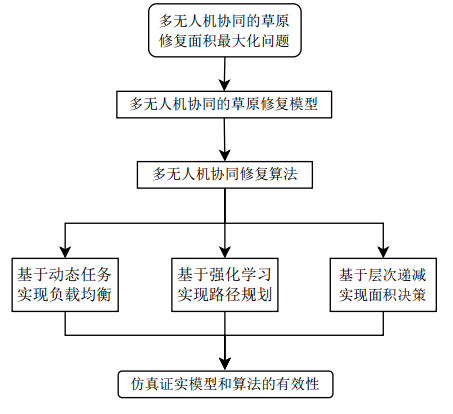
\includegraphics[height=6cm]{主要研究内容.png}
        \caption{主要研究内容}
        \label{fig:my_label}
    \end{figure}
\end{frame}
% \begin{frame}{Pareto Dominance}
% \begin{figure}[!h]
%     \centering
%     \includegraphics[height=6cm]{PD.png}
%     \caption{Pareto Dominance}
%     \label{fig:my_label}
% \end{figure}
% Point A dominates B, Points A, C, D, are nondominated to each
% other.
% \end{frame}

\section{问题建模}
\subsection{多无人机协同的草原修复问题}
\begin{frame}{多无人机协同的草原修复问题}
    % \begin{itemize}
    %     \item {Weighted Sum Approach:}
    %     \begin{align}
    %         \centering 
    %         maximize\ g^{\omega A}(x|\lambda)=\sum_{i=1}^{m} \lambda_if_i(x),subject\;to\;x\in \omega
    %     \end{align}
    %     \item{Tchebycheff Approach:}
    %     \begin{align}
    %         \centering 
    %         minimize\ g^{te}(x|\lambda,z^*)=max_{1\leq i \leq m}\{\lambda_i \lvert f_i(x)-z_i^* \rvert \} 
    %     \end{align}
    %     \item{Boundary Intersection (BI) Approach:}
    %     \begin{align}
    %         \centering 
    %         minimize\ g^{bi}(x|\lambda,z^*)=d,subject\; to\;z^*-F(x)=d\lambda,x \in \Omega
    %     \end{align}
    % \end{itemize}

    \begin{figure}[!h]
        \centering
        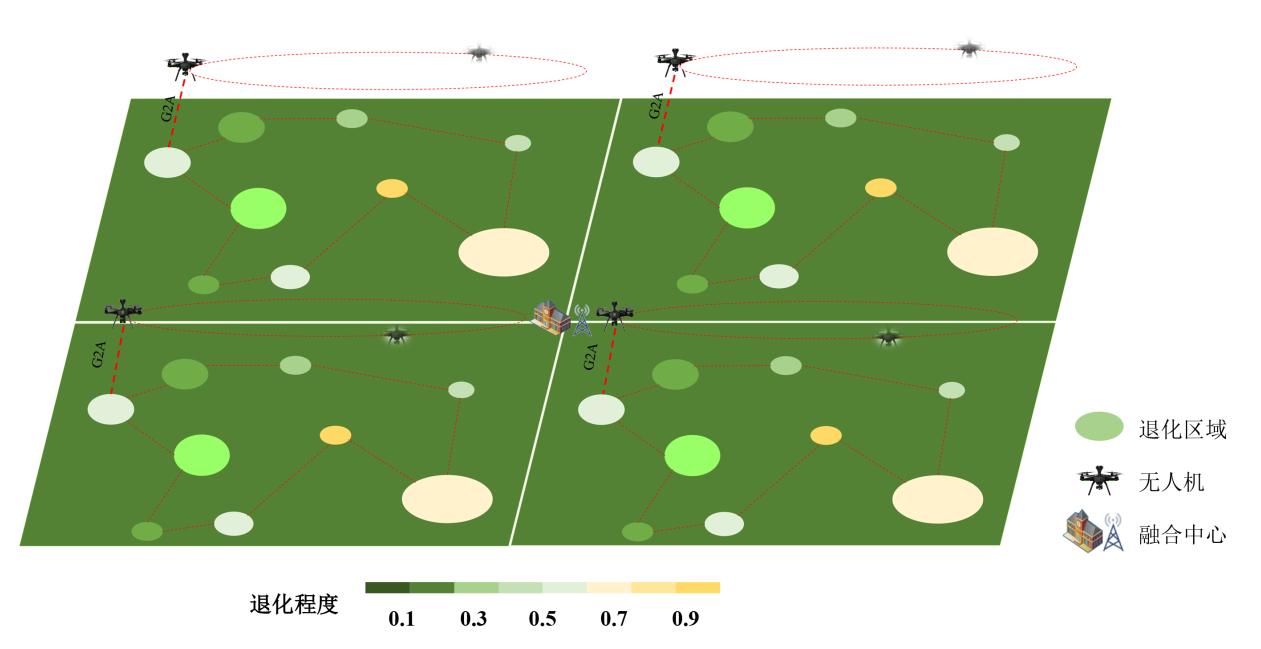
\includegraphics[height=6cm]{多无人机修复退化区域实例.png}
        \caption{多无人机修复退化区域实例}
        \label{fig:my_label}
    \end{figure}
\end{frame}
\subsection{多无人机协同的草原修复面积最大化模型}
\begin{frame}{多无人机协同的草原修复面积最大化模型}
    % \begin{itemize}
    %     \item 退化程度,描述草地退化程度的评分$l_i$。
    %     \item 修复面积, ci 来表示第 i 个退化区域内的单位圆总数。
    %     \item 无人机能耗,无人机所携带的总能量记为$E_{max}$。
    %           \begin{itemize}
    %               \item 无人机修复能耗,$E^{S}$。
    %               \item 无人机信息收集能耗, $E^{ap}$。
    %               \item 无人机飞行能耗, $E^f$。
    %           \end{itemize}
    % \end{itemize}
    \begin{tabular}{cccccc}
   \toprule
   序号 & 姓名 & 性别 & 年龄 & 身高/cm & 体重/kg \\
   \midrule
   1 & 张三 & M & 16 & 163 & 50 \\
   2 & 王红 & F & 15 & 159 & 47 \\
   3 & 李二 & M & 17 & 165 & 52 \\
   \bottomrule
\end{tabular}
\end{frame}

\begin{frame}{无人机能耗}
    \small
    无人机修复能耗:
    \begin{align}
        & e_i^S = \eta q_i, \\
        & q_i=(1+l_i)^\gamma \\
        & E^{S}_u=\sum \limits_{i=1}^Nx_{iu}\omega_{iu}e_i^S
    \end{align}
    % \end{align}
    % \begin{align}
    % \end{align}
    
    % \begin{align}
    无人机信息收集能耗:
    \begin{align}
    & E_u^{ap}=e^{ap}\sum \limits_{i=1}^Nx_{iu}c_i
    \end{align}
    无人机飞行能耗:
    \begin{align}
%          y_{iju}=
% \begin{cases}
% 1& 路径(v_i,v_j\\
% 0& \text{}
% \end{cases}
& E_u^f=e^f\sum \limits_{i=0}^N\sum \limits_{j=0}^Ny_{iju}d_i^j,i\neq j,\\
& e^f=\mathbb{M}\sqrt{\frac{g^3}{2\rho\zeta h}}
\end{align}

\end{frame}
% \begin{frame}{多无人机协同的草原修复面积最大化模型}
% \begin{align}
%         \centering 
%         minimize\ g^{te}(x|\lambda,z^*)=max_{1\leq i \leq m}\{\lambda_i \lvert f_i(x)-z_i^* \rvert \} 
%     \end{align}
% \begin{figure}[!h]
%     \centering
%     
\includegraphics[height=3cm]{c.png}
%     \caption{Tchebycheff Approach in two functions MOP.}
%     \label{fig:my_label}
% \end{figure}
% Where $z = (z_1, . . . , z_m)$ is a reference point.
%     \end{frame}
%     \begin{frame}{Boundary Intersection (BI) Approach}
%         \begin{align}
%         BI:
%             & minimize\ g^{bi}(x|\lambda,z^*)=d, \ subject\; to\;z^*-F(x)=d\lambda,x \in \Omega 
%         \end{align}
%         \begin{align}
%         PBI:
%             & minimize\ g^{bip}(x|\lambda,z^*)=d_1+ \theta d_2 \ subject\; to\; x\in \Omega  \\  
%             & where \ d_1=\frac{||(z^*-F(x))^T\lambda ||}{|| F(x)-(z^*-d_1\lambda)||} \ and \ d_2=||F(x)-(z^*-d_1\lambda)||.
%         \end{align}

% \begin{figure}[!h]
%     \centering
%     \includegraphics[height=3cm]{BI.png}
%     \includegraphics[height=3cm]{PBI.png}
%     \caption{BI and PBI Approach in two functions MOP.}
%     \label{fig:my_label}
% \end{figure}


% \end{frame}
%     \begin{frame}{Framework of MOEA/D}
%     At each generation, MOEA/D with the Tchebycheff approach maintains:
%     \begin{itemize}
%         \item A population of N points , where $x^i$ is the current solution to the i th subproblem.
%         \item $FV^1,...,FV^N$,where $FV^i$ is the F-value of $x^i$. $FV^i=F(x^i) for\;each\;i=1,...,N$.
%         \item $z=(z_1,z_2,...,z_m)^T$,where $z_i$ is the best value found so far for objective $f_i$.
%         \item An external population (EP), which is used to store non-
% dominated solutions found during the search.
%     \end{itemize}
%     \end{frame}
%     \begin{frame}{Flow Chart}
% \begin{figure}
% \centering
% \begin{tikzpicture}[node distance=1cm]
% \node (input1) [io,yshift=0.2cm] {Input:{EP,N,$\lambda$,T}};
% \node (process1) [process,below of=input1,yshift=0.2cm] {Initialization};
% \node (process2) [process,below of=process1,yshift=0.2cm] {i=1};
% \node (process3) [process,below of=process2,yshift=0.2cm] {Reproduction};
% \node (process4) [process,below of=process3,yshift=0.2cm] {Update};
% \node (decision0) [decision,below of=process4,yshift=-0.1cm] {i>N?};
% \node (decision1) [decision,right of=decision0,xshift=3.25cm] {Stopping Criteria?};
% \node (process2b) [process,left of=decision0,xshift=-2.5cm] {i+=1};
% \node (output) [io,below of=decision1,yshift=-1cm] {Output:EP};

% \draw [arrow] (input1) -- (process1);
% \draw [arrow] (process1) -- (process2);
% \draw [arrow] (process2) -- (process3);
% \draw [arrow] (process3) -- (process4);
% \draw [arrow] (process4) -- (decision0);
% \draw [arrow] (decision0) -- node[anchor=south] {yes} (decision1);
% \draw [arrow] (decision0) -- node[anchor=south] {no} (process2b);
% \draw [arrow] (decision1) -- node[anchor=east] {yes} (output);
% \draw [arrow] (decision1) |- node[anchor=south] {no} (process2);
% \draw [arrow] (process2b) |- (process3);
% \end{tikzpicture}

% \caption{Flow chart}
% \label{fig:my_label}
% \end{figure}
%     \begin{figure}[!h]
%     \centering
%     \includegraphics[height=7cm]{flow.png}
%     % \includegraphics[height=3cm]{PBI.png}
%     \caption{Flowchart of MOEA/D algorithm}
%     \label{fig:my_label}
% \end{figure}
%     \end{frame}







% \begin{frame}{Algorithm Initialization}
% \begin{itemize}
%     \item Set  EP  = $\phi$.
%     \item Compute the Euclidean distances between any two weight vectors and then work out the T closest weight vectors to each weight vector. for each i = 1,...,N,set $B(i)={i_1,...,i_T}$,where $\lambda^{i_1},...,\lambda^{i_T}$ are the T closet weight vectors to $\lambda^i$.
%     \item  Generate an initial population $x^i,...,x^N$ randomly or by a problem-specific method.Set $FV^i = F(x^i)$.
%     \item  Initialize $z=(z_1,...,z_m)^T$ by a problem-specific method.

% \end{itemize}
% \end{frame}
% \begin{frame}{Algorithm Update}
% For $i = 1,...,N$ do:
% \begin{itemize}
%     \item Reproduction:Randomly select two indexes:k,l from B(i),and then generate a new solution $y$ from $x^k$ and $x^l$ by using genetic method.
%     \item Improvement:Apply a problem-specific repair/improvement heuristic on $y$ to produce $y^'$.
%     \item Update of $z$:For each $j = 1,...,m$,if $z_j<f_j(y')$, then set $z_j=f_j(y')$.
%     \item Update of Neighboring Solutions:for each index $j \in B(i)$,if $g^{te}(y'|\lambda^j,z)\leq g^{te}(x^j|\lambda^j,z)$,then set $x^j=y'$ and $FV^j=F(y')$.
%     \item Update of EP:\\Remove from all the vectors dominated by $F(y')$.\\Add $F(y')$ to EP if no vectors in EP dominate $F(y')$.
% \end{itemize}
% Stopping Criteria:\\
% \centerline{If stopping criteria is satisfied,then stop and output .} 
% \end{frame}


% \begin{frame}{调度算法}
% \begin{algorithm}[H]
%   \SetAlgoLined
%   % \big
%   \tiny
%   % \KwIn{MOP (1),N,\lambda^i ,T,a \; stopping \; criterion}
%   \KwIn{参数序列Parms,无人机修复地图集合M_u,无人机状态集合S_u。}
%   \KwOut{无人机访问的节点序列O_p,无人机修复的面积O_a,无人机剩余能量O_e。}
%   {$P_u^{self} = FlyToPoint(P_u^{near0})$}\\
%   % {Initialize the reference point $z^*$ as $z^*_j=min_{1\leq i \leq N}f_j(x^i)$;}\\
%   \While{$M_u \neq \; \varnothing $}{
%     % \For{$i=1$ to $N$}{
%     %     \For{randomly select k,l in B(i)}{
%     %         {generate a new solution y from $x^k$ and $x^l$.}\\
%     %         {improve $y$ to produce $y'$}\\
%     %         \For{$j=1$ to $m$}{
%     %             \If {$z_j$<$f_j(y')$}{
%     %                 $z_j=f_j(y')$
%     %             }
%     %         }
%     %         \For{each j in B(i)}{
%     %             \If{$g^{te}(y'|\lambda^j,z)\leq g^{te}(x^j|\lambda^j,z)$}{
%     %                 {$x^j=y'$}\\
%     %                 {$FV^j=F(y')$}
%     %             }
%     %         }
%     %         {Remove from all the vectors dominated by $F(y')$}\\
%     %         {Add $F(y')$ to if no vectors in $EP$ dominate $F(y')$.}
%     %     }
%     % }
%         {$E_u^{r1}$ = PlaningPath(M_u,$P_u^{self}$)}\\
%         {SendToCenter(S_u,M_u,$E_u^{r1}$)}\\
%         {$M_u^{temp}$ = updateMap(M^{global},$P_u^{self}$)}\\
%         {$RecvToUAV(M_u^{tmp})$}\\
%         {$E_u^{r1} = PlaningPath(M_u^{tmp},P_u^{self})$}\\
%         {$SendToCenter(E_u^{r2})$}\\
%         \If{$\sum_{u=1}^UE_u^{r2}\geq\sum_{u=1}^UE_u^{r1}}{
%             {$RecvToUAV(M_u^{tmp})$}\\
%             {$M_u = M_u^{tmp}$}
%         }
%         {$\sigma = DecideArea(E_u^r,M_u)$}\\
%         {$ActionUAV(\sigma_{ui},c_i,P_u^{self})$}\\
%         {$DropPointFromMap(M_u,P_u^{self})$}\\
%         {$P_u^{self} = FlyToPoin(P_u^{benefit})$}
% }   
% {FlyToPoint(P_u^0)}
% \caption{MOEAD}
% \end{algorithm}




% \begin{frame}{Updating}
%     \begin{figure}
%         \centering
%         \includegraphics[height=7cm]{Update.png}
%         \caption{Updating Graph.}
%         \label{fig:my_label}
%     \end{figure}
% \end{frame}
\subsection{数学模型}
\begin{frame}{数学模型}
    \scriptsize

    % 总面积表示:
    该问题可被描述为:
    \begin{align}
          % & C^T = \sum_{u=1}^U \sum_{i=1}^N x_{iu} \sigma_{iu}\\
    % \end{align}
    % \begin{align}
        \mathop{\max}_{x_{iu},\sigma_{iu}} & C^T = \sum_{u=1}^U \sum_{i=1}^N x_{iu} \sigma_{iu}                              \\
        \mathrm{s.t.}                      & E_u^S+E_u^{ap}+E_u^f \leq E_{max} u \in U                                       \\
                                           & \sum_{j=1}^Ny_{0ju}=\sum_{i=1}^Ny_{i0u}=1,u \in U                               \\
                                           & \sum_{j=1}^Ny_{jiu}=\sum_{j=1}^Ny_{iju}=x_{iu},\forall{i \in M,u\in U,j \neq i} \\
                                           & \sum_{u=1}^Ux_{iu}=1,\forall{i \in M}                                           \\
                                           & 1\leq \sigma_{iu} \leq c_i,                                                     \\
                                           & y_{iju}\in \lbrace0,1\rbrace,                                                   \\
                                           & x_{iu}\in \lbrace0,1\rbrace
    \end{align}
    % \tiny
    % \begin{align}
    %     &ZDT1:f_1(x)=x_1;f_2(x)=g(x) \left[ 1-\sqrt{\frac{f_1(x)}{g(x)}} \right];where \;g(x)=1+\frac{9(\sum_{i=2}^nx_i)}{(n-1)}\\
    %     &ZDT2:f_1(x)=x_1;f_2(x)=g(x) \left[ 1-(\frac{f_1(x)}{g(x)})^2 \right]\\
    %     &ZDT3:f_1(x)=x_1;f_2(x)=g(x) \left[ 1-\sqrt{\frac{f_1(x)}{g(x)}}-\frac{f_1(x)}{g(x)}\sin{(10\pi x_1)} \right]\\
    %     &ZDT4:f_1(x)=x_1;f_2(x)=g(x) \left[ 1-\sqrt{\frac{f_1(x)}{g(x)}} \right];where \;g(x)=1+10(n-1)+\sum_{i=2}^n\left[ x_i^2-10\cos{(4\pi x_i)}\right ]\\
    %     &DTLZ1:f_1(x)=(1+g(x))x_1x_2;f_2(x)=(1+g(x))x_1(1-x_2);f_3(x)=(1+g(x))(1-x_1)\\
    %     &\ \ \ \ \ \ \ \ \ \ \ \ where\;g(x)=100(n-2)+100\sum_{i=3}^n{ (x_i-0.5)^2-\cos{\left[ 20\pi(x_i-0.5)\right ]}}\\
    %     &DTLZ2:f_1(x)=(1+g(x))\cos{(\frac{x_1\pi}{2})}\cos{(\frac{x_2\pi}{2})};f_2(x)=(1+g(x))\cos{(\frac{x_1\pi}{2})}\sin{(\frac{x_2\pi}{2})};f_3(x)=(1+g(x))\sin{(\frac{x_1\pi}{2})}\\
    %     &\ \ \ \ \ \ \ \ \ \ \ \ where \; g(x)=\sum_{i=3}^nx_i^2
    % \end{align}
\end{frame}


%     \begin{frame}{ZDT Tset}
%         \begin{figure}[htbp]
%         \centering
%         \includegraphics[height=3.3cm]{ZDT1.png}
%         \includegraphics[height=3.3cm]{ZDT2.png}
%         \includegraphics[height=3.3cm]{ZDT3.png}
%         \includegraphics[height=3.3cm]{ZDT4.png}
%         \caption{Two-dimensional test function in using MOEA/D by Tchebycheff Approach.}
%         \label{mylabel}
%         \end{figure}
%     \end{frame}
%     \begin{frame}{DTLZ Test}
%     \begin{figure}[htbp]
%         \centering
%         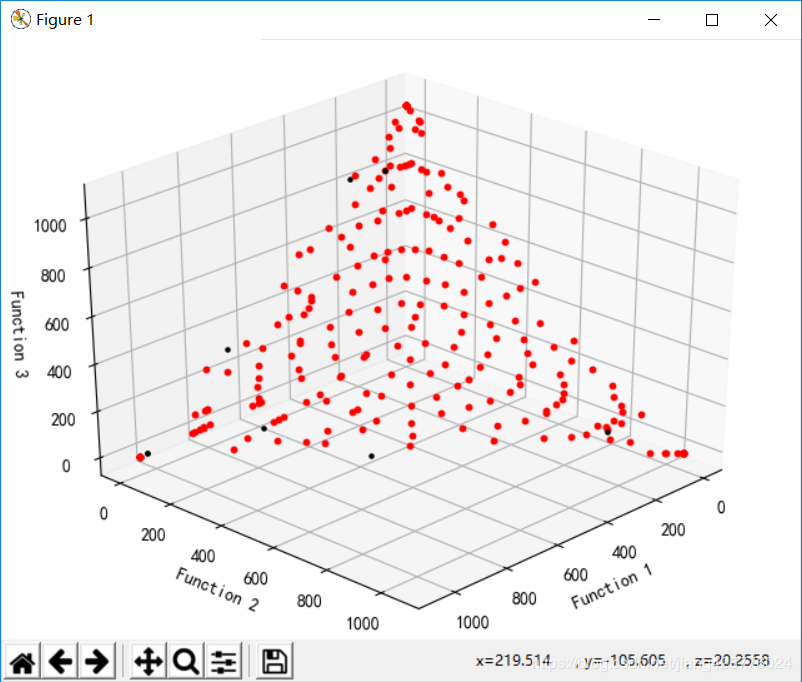
\includegraphics[height=3cm]{DTLZ1.png}
%         \includegraphics[height=3cm]{DTLZ2.png}
%         \caption{DTZL with m=3 in MOEA/D by Tchebycheff Approach.}
%         \label{mylabel}
%     \end{figure}

%         \begin{figure}[!h]
%     \centering
%     \includegraphics[height=3cm]{PBIDTZL1.png}
%     \includegraphics[height=3cm]{PBIDTZL2.png}
%     \caption{DTZL with m=3 in MOEA/D by PBI Approach.}
%     \label{fig:my_label}
% \end{figure}

%     \end{frame}
% \section{Comparison}
% \subsection{Two Performance Indexes}
%     \begin{frame}{Two Performance Indexes}
%     \begin{itemize}
%         \item (C-metric)Let A and B be two approximations to the PF of a MOP ,C(A,B) is defined as the percentage of the solutions in B that are dominated by at least one solution in A.
%         \begin{align}
%             \centering 
%             C(A,B)=\frac{\lvert \{\mu\in B|\exists\nu \in A:\nu\; dominates\;\mu \lvert}{\lvert B\rvert}
%         \end{align}
%         \item(D-metric)Let $P^*$ be a set of uniformly distributed points along the PF. Let A be an approximation to the PF, the average distance from $P^*$ to A is defined as.
%         \begin{align}
%             \centering 
%             D(A,P^*)=\frac{\sum_{\nu \in P^*} d(\nu,A)}{\lvert P^*\rvert}
%         \end{align}
%         $d(\nu,A)$ is the minimum Euclidean distance between $\nu$ and the point in A.
%     \end{itemize}
%     \end{frame}
% \subsection{Comparsion With MOGLS}
%     \begin{frame}{C-metric and D-metric}
%         \begin{figure}
%             \centering
%             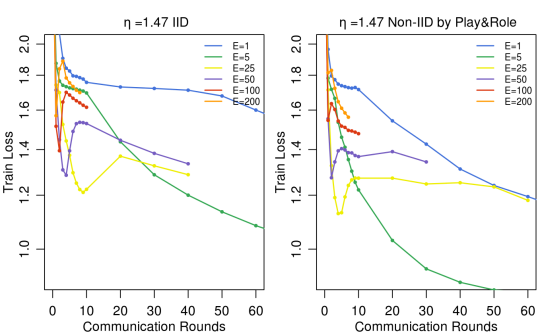
\includegraphics[width=7.6cm,height=3cm]{table3.png}
%             \caption{\small Set coverage between MOEA/D(A) and MOGLS(B).}
%             \label{fig:my_label}
%         \end{figure}
%         \begin{figure}
%             \centering
%             \includegraphics[width=8cm,height=3cm]{table4.png}
%             \caption{\small D-metric values of MOEA/D and MOGLS.}
%             \label{fig:my_label}
%         \end{figure}
%         \small D-METRIC of MOEA/D is lower than that of MOGLS
%     \end{frame}
%     \begin{frame}{Comparsion and Discussion}
%     \begin{figure}
%         \centering
%         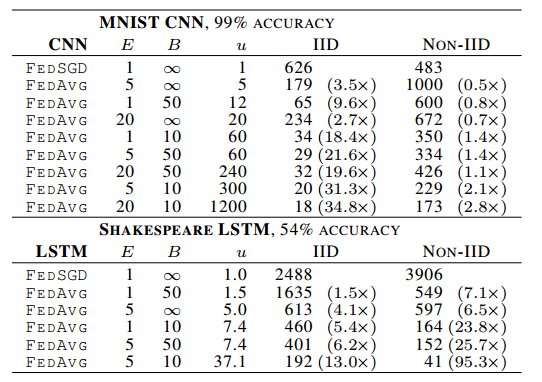
\includegraphics[width=8cm,height=4cm]{table2.png}
%         \caption{Avergae CPU time (in seconds) used by MOEA/D and MOGLS.}
%         \label{fig:my_label}
%     \end{figure}
%     From these tables, we can claim that MOEA/D is computationally much cheaper and can produce better approximations than MOGLS.
%     \end{frame}
\section{求解方法}
\subsection{基于强化学习的最优路径规划}
\begin{frame}{问题建模}
    % \begin{itemize}
    %     \item 状态,$t(<i),i\in [1,n+1]$
    %     \item 动作,$t(i)=(v_{i-1},v_i)$
    %     \item 状态转移函数,$T(t(<i)|t(i))=t(<i+1),i\in [1,n]$
    %     \item 随机策略函数,$p(t|V)=\prod \limits_{i=1}^np((t(i)|t(<i))$
    %     \item 即时奖励,$r(t(<i)|t(i))=d_{i-1}^i+\beta \frac{\sum \limits_{j=1}^{\lceil i/2 \rceil}l_j}{\sum \limits_{j=1}^il_j}$
    %     \item 最终回报,$R(t|V)=d_n^0+\sum \limits_{i=0}^{n-1}+\beta \frac{\sum \limits_{j=1}^{\lceil i/2 \rceil}l_j}{\sum \limits_{j=1}^il_j}$
    %     % \item 环境。
    % \end{itemize}
    \begin{align}
        \text{状态}:&t(<i),i\in [1,n+1]\\
        \text{动作}:&t(i)=(v_{i-1},v_i)\\
        \text{状态转移函数}:&T(t(<i)|t(i))=t(<i+1),i\in [1,n]\\
        \text{随机策略函数}:&p(t|V)=\prod \limits_{i=1}^np((t(i)|t(<i))\\
        \text{即时奖励}:&r(t(<i)|t(i))=d_{i-1}^i+\beta \frac{\sum \limits_{j=1}^{\lceil i/2 \rceil}l_j}{\sum \limits_{j=1}^il_j}\\
        \text{最终回报}:&R(t|V)=d_n^0+\sum \limits_{i=0}^{n-1}+\beta \frac{\sum \limits_{j=1}^{\lceil i/2 \rceil}l_j}{\sum \limits_{j=1}^il_j}
    \end{align}
\end{frame}
\begin{frame}{网络结构}
    \begin{figure}[!h]
        \centering
        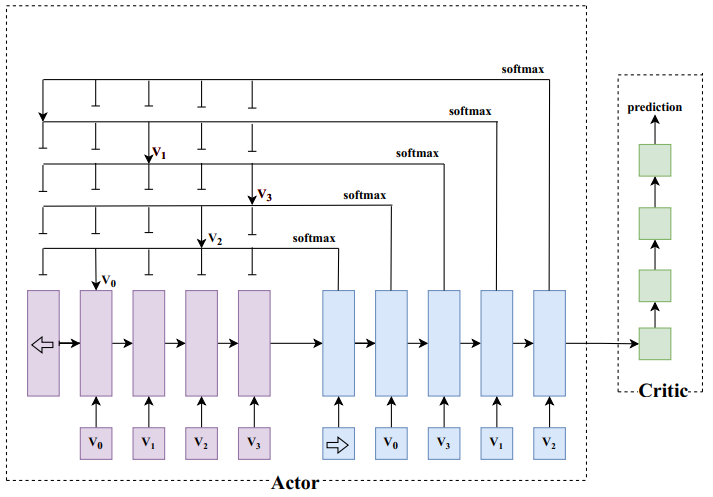
\includegraphics[height=7cm]{网络结构图.png}
        \caption{网络结构图}
        \label{fig:my_label}
    \end{figure}
\end{frame}

\begin{frame}{网络目标}

行动者网络:
\begin{align}
    &J(\theta|V) = \mathbb{E}_{t\sim p_\theta(.|V)}R(t|V)\\
    &\nabla_ \theta J(\theta|V)=\mathbb{E}_{t\sim p_\theta(.|V)}[(R(t|V)-b(V))\nabla_\theta(t|V)\log_{p_\theta}(t|V)]\\
    &\nabla_ \theta J(\theta)\approx \frac{1}{B}\sum \limits_{i=1}^B(R(t|V_i)-b(V_i))\nabla_ \theta \log_{p_\theta }(t_i|V_i)
\end{align}

评论家网络:
\begin{align}
    &L(\theta_c|V)=\frac{1}{B}\sum \limits_{i=1}^B \Vert b_\theta_c(V_i)-R(t_i|V_i)\Vert_2^2
\end{align}
\end{frame}
\subsection{多无人机协同调度算法}
\begin{frame}{协同调度算法}
    \begin{figure}[!h]
        \centering
        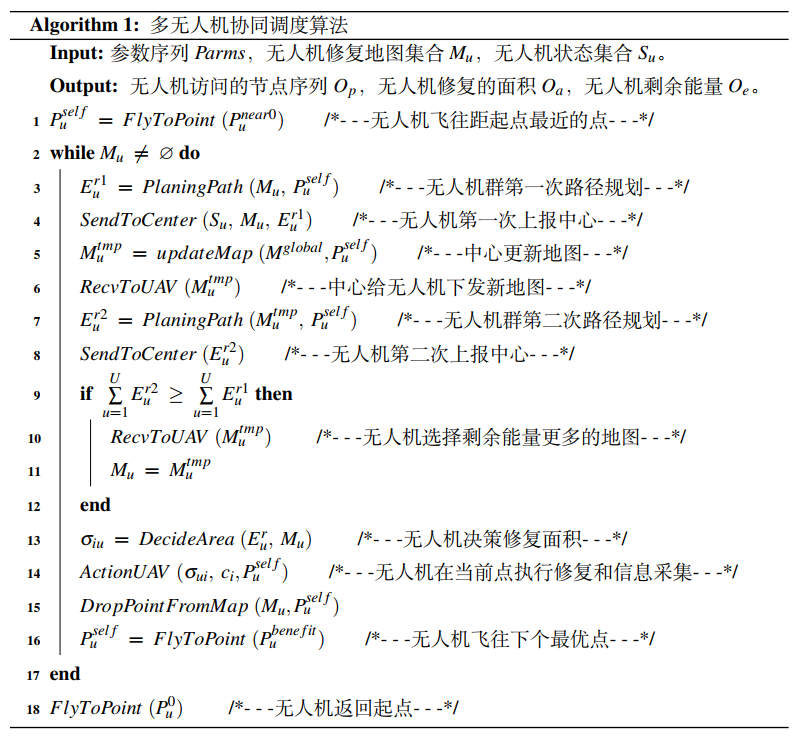
\includegraphics[height=7.5cm]{调度算法.png}
        \caption{多无人机修复退化区域实例}
        \label{fig:my_label}
    \end{figure}
\end{frame}

\section{仿真结果}
% \subsection{仿真环境}
% \begin{frame}{仿真环境}
% \end{frame}
% \subsection{仿真设置}
\begin{frame}{仿真设置}
    \begin{figure}[!h]
        \centering
        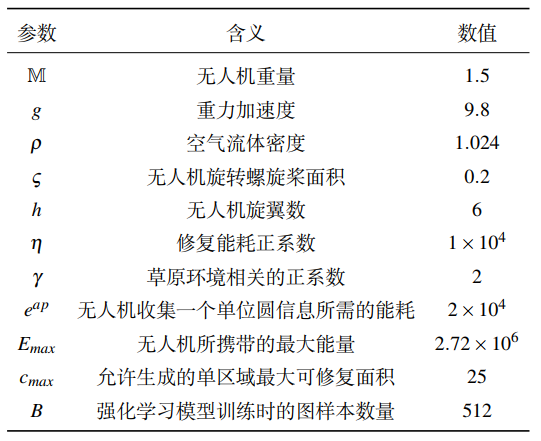
\includegraphics[height=6cm]{仿真参数设置.png}
        \caption{仿真参数设置}
        \label{fig:my_label}
    \end{figure}
\end{frame}
% \subsection{仿真结果}
\begin{frame}{仿真结果}
    \begin{figure}[!h]
        \centering
        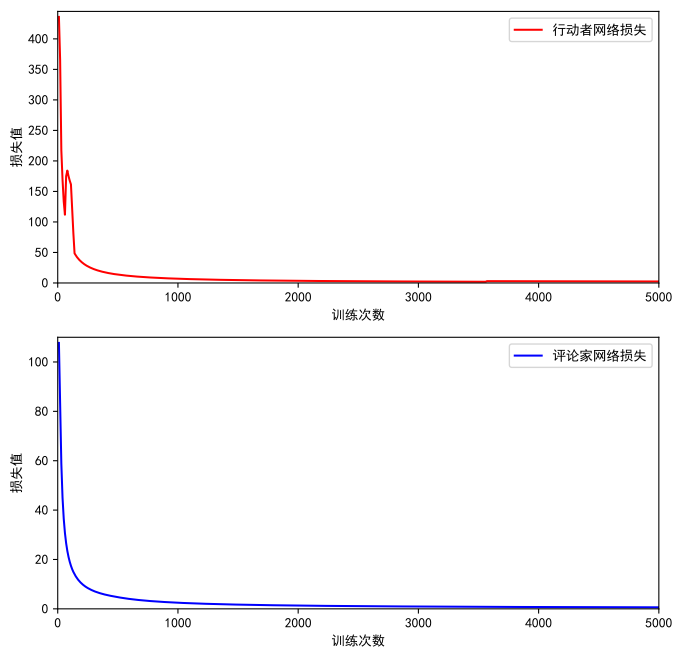
\includegraphics[height=6cm]{模拟训练过程.png}
        \caption{模拟训练过程}
        \label{fig:my_label}
    \end{figure}
\end{frame}

\begin{frame}{无人机修复详情}
    \begin{figure}[!h]
        \centering
        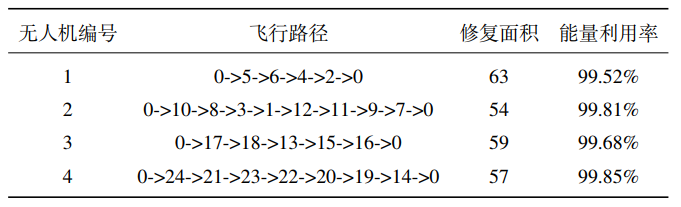
\includegraphics[height=3cm]{无人机修复详情.png}
        \caption{无人机修复详情}
        \label{fig:my_label}
    \end{figure}
\end{frame}

\begin{frame}{无人机修复轨迹}
    \begin{figure}[!h]
        \centering
        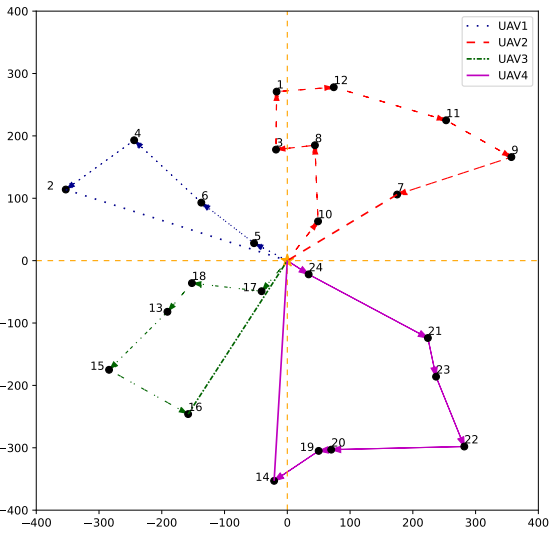
\includegraphics[height=7cm]{无人机修复轨迹.png}
        \caption{无人机修复轨迹}
        \label{fig:my_label}
    \end{figure}
\end{frame}

% \begin{frame}{参考论文}
% 	\printbibliography
% \end{frame}

\begin{frame}[plain,t]
    \vspace{100pt}
    \centering
    {\Huge Thanks for your time!\\Q\&A}
\end{frame}
\end{document}